\chapter{The Wu Experiment}
\label{cha:wu_exp}

The Wu experiment focuses on the parity transformation $\hat P$, charge conjugation transformation $\hat C$ and its combination $\hat C\hat P$.
In physics, parity describes the symmetry of spatial coordinates.
A given point $(t, \vec x)$ would transform to $(t, -\vec x)$ under $\hat P$.
Classical physics is invariant under parity transformation thus conserving parity.
The intrinsic parity of a particle is calculated via the spin $l$ by $ \hat P=(-1)^l$.
As classical physics is invariant under the change of sign in spatial coordinates, it is also invariant under the change of sign of electric charges.
In elementary particle physics, the change of sign of electric charges is called charge conjugation transformation $\hat C$ converting particles into anti-particles and vice versa, $\hat C \ket{e} = \ket{\bar e}$.
By 1957, significant discoveries in particle physics had already taken place, such as $e^\pm,\ \nu_e,\ \mu, p, \gamma,\ \pi$ and $K$.
Parity conservation was evident for the electromagnetic (EM), the strong and the gravitational interaction, but there was no experimental evidence for parity conservation in the weak interaction \cite{CaseStudies}.
For most physicists, it seemed self-evident that parity is conserved in the weak interaction as well.
In 1956 however, Tsung-Dao Lee (*1926) and Chen Ning Yang (*1922) considered the conservation of $\hat P$ in the weak interaction and proposed different experiments to test it  \cite{PhysRev.104.254}.
\begin{wrapfigure}{r}{5.5cm}
    \centering
    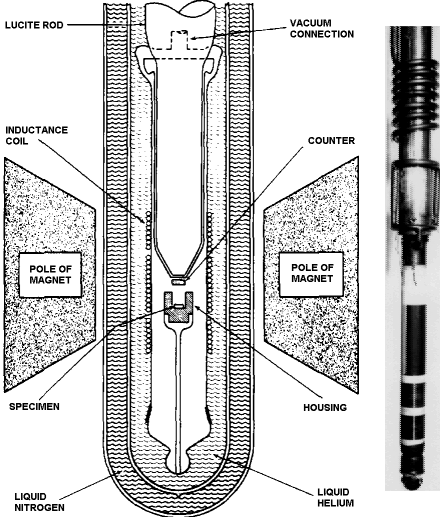
\includegraphics[width=0.35\textwidth]{figs/setup.png}
    \caption{Schematic illustration and photograph of the apparatus \cite{NIST}.}
    \label{fig:setup}
\end{wrapfigure}
The first to carry out such an experiment was Chien-Shiung Wu (1912-1997) when she was approached by Lee and Yang for her expertise in $\beta$-decay in 1956.
The experiment was based on the decay of Cobalt via $\cobalt\rightarrow \nickel+e^-+2\gamma+\bar\nu_e$.
Cobalt has a spin of 5 and was used because it decays via a $\beta$-decay into excited nickel with a spin of 4 meaning that the particles have to have the same spin direction.
Due to the polarization of the nucleus, the electrons are emitted either upwards or downwards.
The emission of the electrons is invariant under parity transformation if it is conserved in the weak interaction and vice versa.
A cerium magnesium nitrate (CMN)-crystal with a small layer of cobalt was used as the specimen and placed inside a housing necessary to hold the polarization \cite{CaseStudies} which was caused by a magnetic field.
A schematic illustration with a photograph of the used apparatus is shown in figure \ref{fig:setup}.
\begin{wrapfigure}{L}{5.5cm}
    \centering
    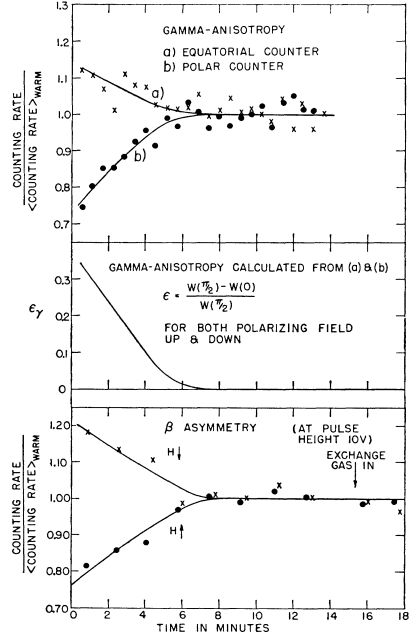
\includegraphics[width=0.4\textwidth]{figs/resultsWu.png}
    \caption{Measured results showing the gamma anisotropy and electron asymmetry for a polarizing magnetic field pointing up and down \cite{PhysRev.105.1413}.}
    \label{fig:resultsWu}
\end{wrapfigure}
An anthracene crystal was used as a scintillation counter and placed inside the lucite rod.
Sodium iodide gamma-scintillation counters were installed externally to measure the $\gamma$.
If the magnetic field is repolarized, the electron emission rates will stay the same if parity is conserved.
The $\gamma$-scintillation counters were used to measure the state of the polarization because the originally isotropic emission changes under parity transformation to an oval anisotropy as this is an electromagnetic process that conserves parity \cite{CaseStudies}.
The experimental results are shown in figure \ref{fig:resultsWu}.
The measured electron rates show a clear dependence on the polarization direction.
This asymmetry in the emission of electrons is violating parity conservation proofing \cite{PhysRev.105.1413}.
By comparing the $\gamma$ and $\beta$ emissions for similarities, it can be seen that the $\beta$ asymmetry reduces when the $\gamma$ anisotropy reduces indicating that it is not due to misalignment of the apparatus.
Further systematic checks have been made showing no dependence on systematic uncertainties \cite{CaseStudies}.
Parity nonconservation in the weak interaction also implies the violation of charge conjugation assuming its combination is conserved.

The measured asymmetry was quantified by comparing the $\beta$ asymmetry with the $\gamma$ anisotropy which was difficult as it was difficult to measure the anisotropy.
Thus, only a lower limit of $\alpha\leq -0.7$ could be measured.
A two-component neutrino theory published by Lee and Yang introduces right-handed neutrinos and left-handed antineutrinos which are both massless and lead to an asymmetry of $\alpha=-1$ \cite{PhysRev.105.1671}.
Thus, a new experiment was designed to measure an asymmetry value of $\alpha=\num{-1.01(0.02)}$ which is in perfect agreement with the theory leading to the (V-A)-structure introduced by Richard Feynman and Murray Gell-Mann.
Lee and Yang received a Nobel Prize while Wu did not.
According to the Sakharov conditions (1967) \cite{Gato-Rivera} the matter-antimatter asymmetry in the universe could be explained if, amongst other things, $\hat C$ and $\hat C\hat P$ can be violated which the Wu experiment demonstrated.
The search for $\hat C\hat P$-asymmetry is still researched today as the largest asymmetry yet was measured at LHCb in 2022 \cite{AntiSymmetryLHC}.